%Ukazka zaverecne zpravy
%Posledni zmena 02/2018, Martin Cadik

\documentclass[11pt,a4paper,oneside]{article}
\usepackage[utf8]{inputenc}
\usepackage{a4wide}
\usepackage{url}
\usepackage[breaklinks=true,hidelinks]{hyperref}
%\usepackage[chapter]{algorithm}
%\floatname{algorithm}{Alg.} 
\usepackage{ifpdf}
\ifpdf
\usepackage[pdftex]{graphicx}
\DeclareGraphicsExtensions{.pdf,.png,.gif,.jpg}
\else
\usepackage[final]{graphicx}
\DeclareGraphicsExtensions{.eps,.png,.gif,.jpg}
\fi 
\graphicspath{{fig/}}
\usepackage[export]{adjustbox}



\begin{document}

%Uvodni stranka
\thispagestyle{empty}
\begin{center}
\vspace*{60mm}
{Semestrální projekt předmětu Výpočetní fotogragie -- závěrečná zpráva }\\
\smallskip
{\Large\bf Tone Mapping: implementace algoritmu Khan20}\\
\smallskip
{\it Milan Tichavský, \url{xticha09@fit.vut.cz}}\\
\vfill
{\bf Vedoucí práce:} {\it doc. Ing. Martin Čadík, Ph.D., \url{cadik@fit.vut.cz}} 
\hfill {Květen 2025}


\end{center}
\newpage


%Vlastni zprava
\section{Úvod}
Toto je ukázková kostra závěrečné zprávy pro předmět VYF.



\section{Případná sekce}
Např. nějaká fyziologie vidění apod. -- to, co je nezbytně nutné k pochopení
dalšího textu. V celém dokumentu je třeba správně citovat 
zdroje~\cite{Daly:1993:VDP:197765.197783}.


\section{Popis problému a řešení}
Lze rozdělit i na více sekcí, resp. 

\subsection{Podsekcí}
Příklad obrázku, viz obr.~\ref{fig:vdp}.


\begin{figure}[htb]
  \begin{center}
    \includegraphics{fig/vdp}
    \caption{Popis obrázku} 
    \label{fig:vdp}
  \end{center}
\end{figure}



\section{Implementace}
Popis implementace a vizualizace jednotlivých fází výpočtu.


\section{Výsledky}
Nejdůležitější část -- diskuse výsledků, 
načtené/vypozorované klady a zápory, operační složitost, ...
Ukázkové obrázky.

\begin{tabular}{lll}
    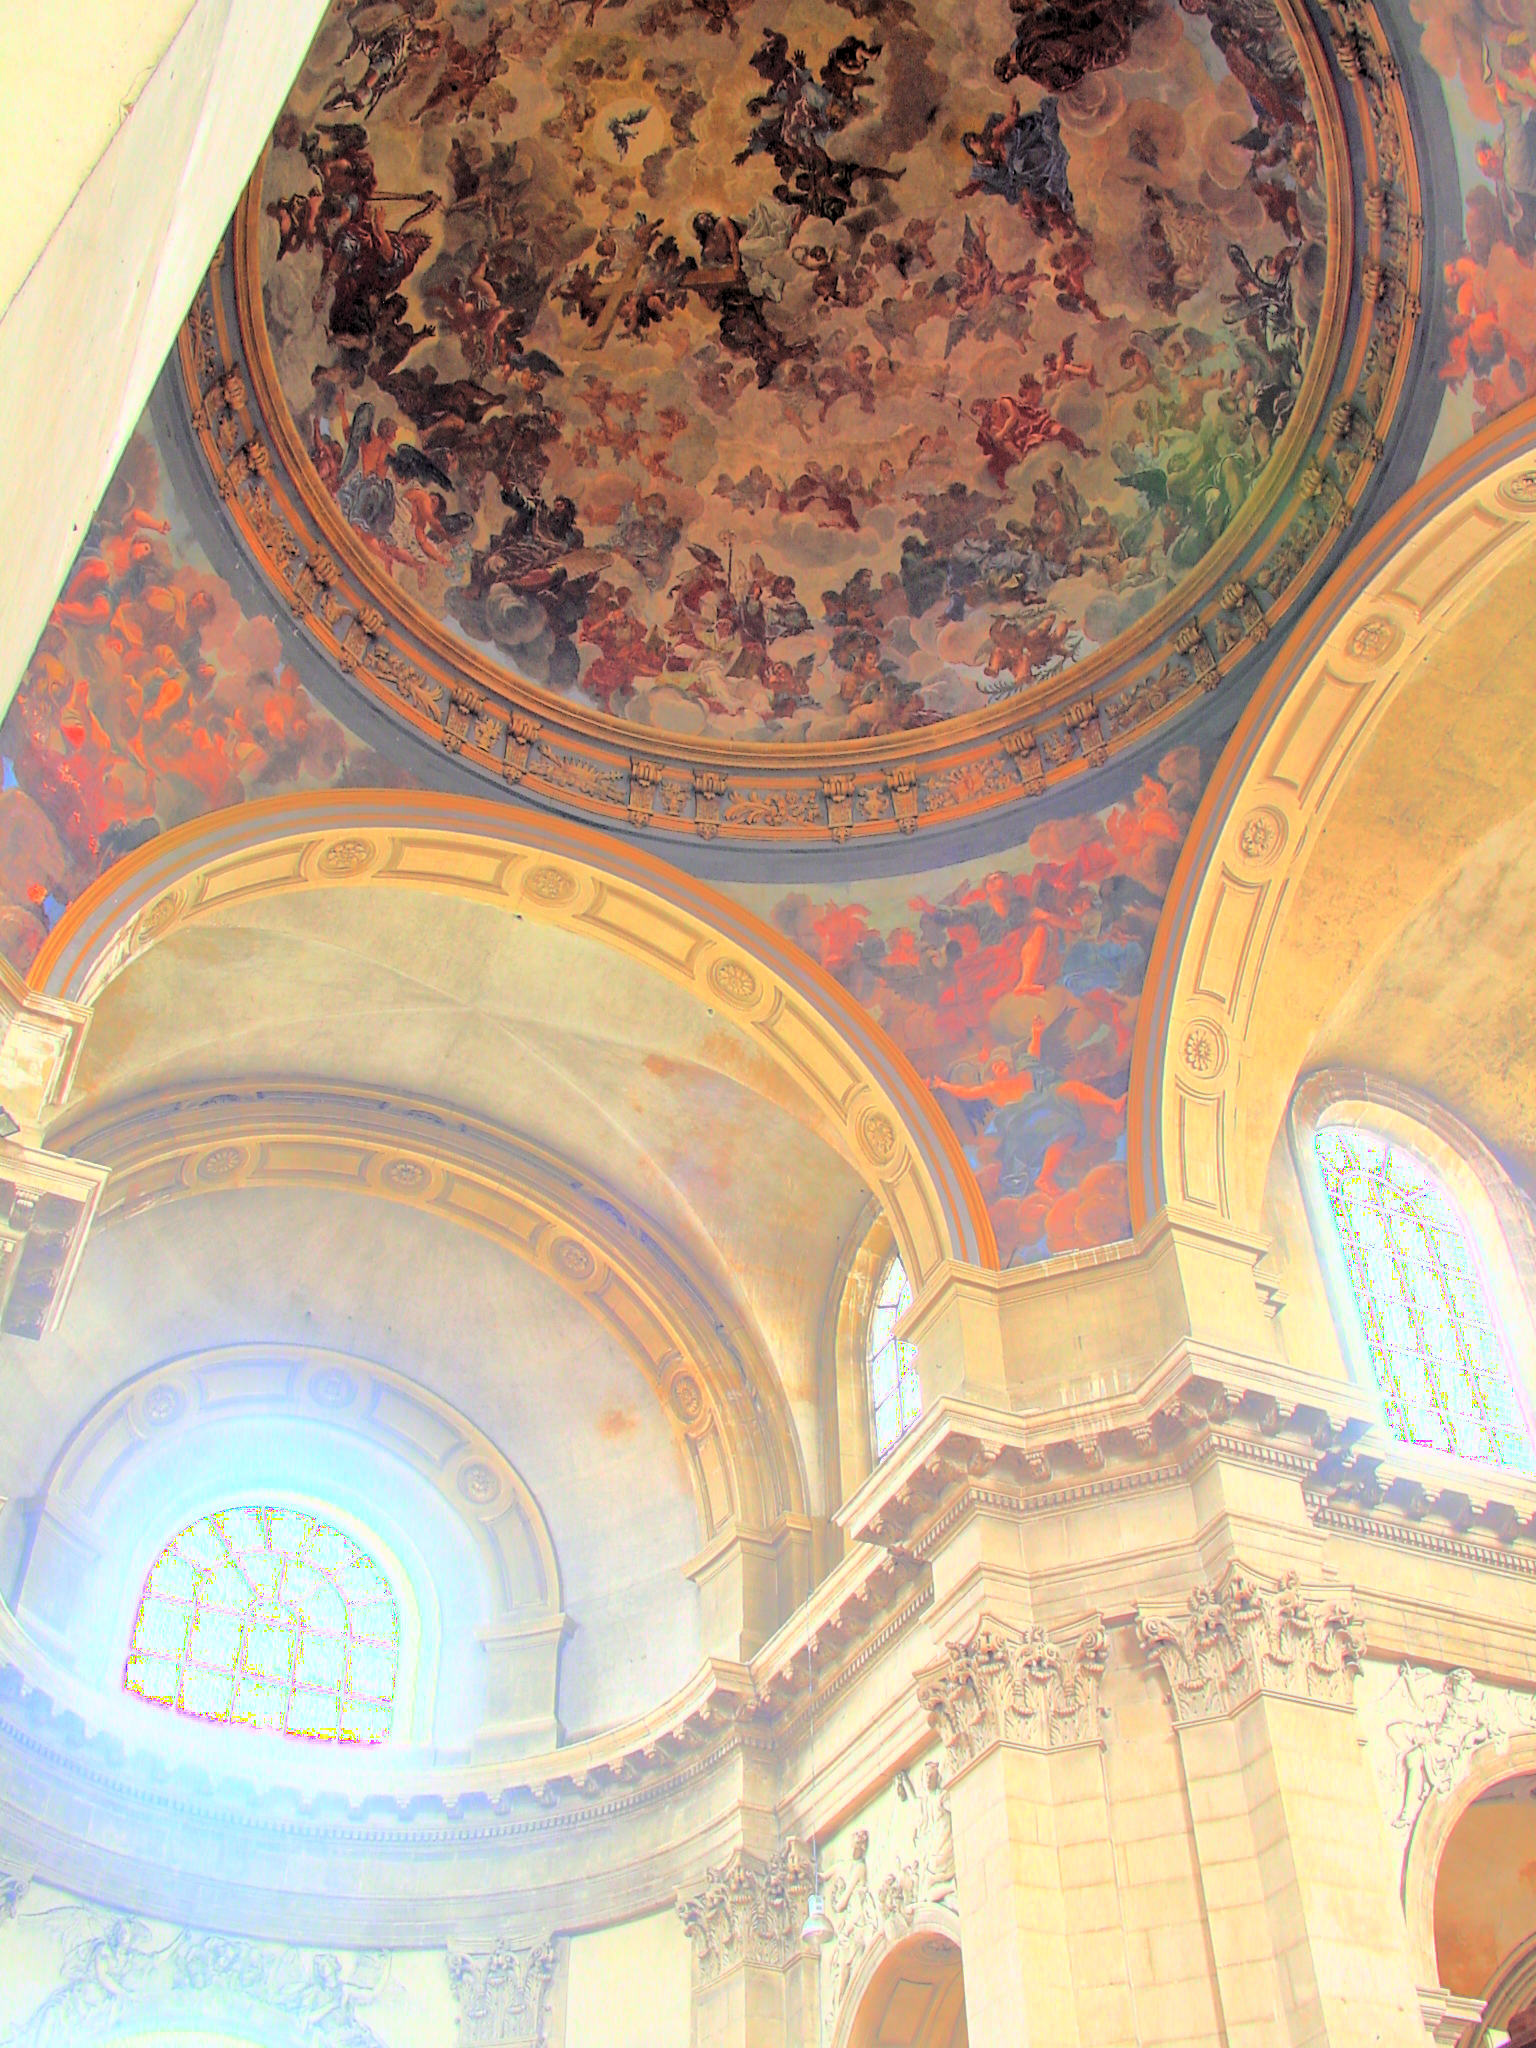
\includegraphics[width=.3\linewidth,valign=m]{churchKhan20.png} &
    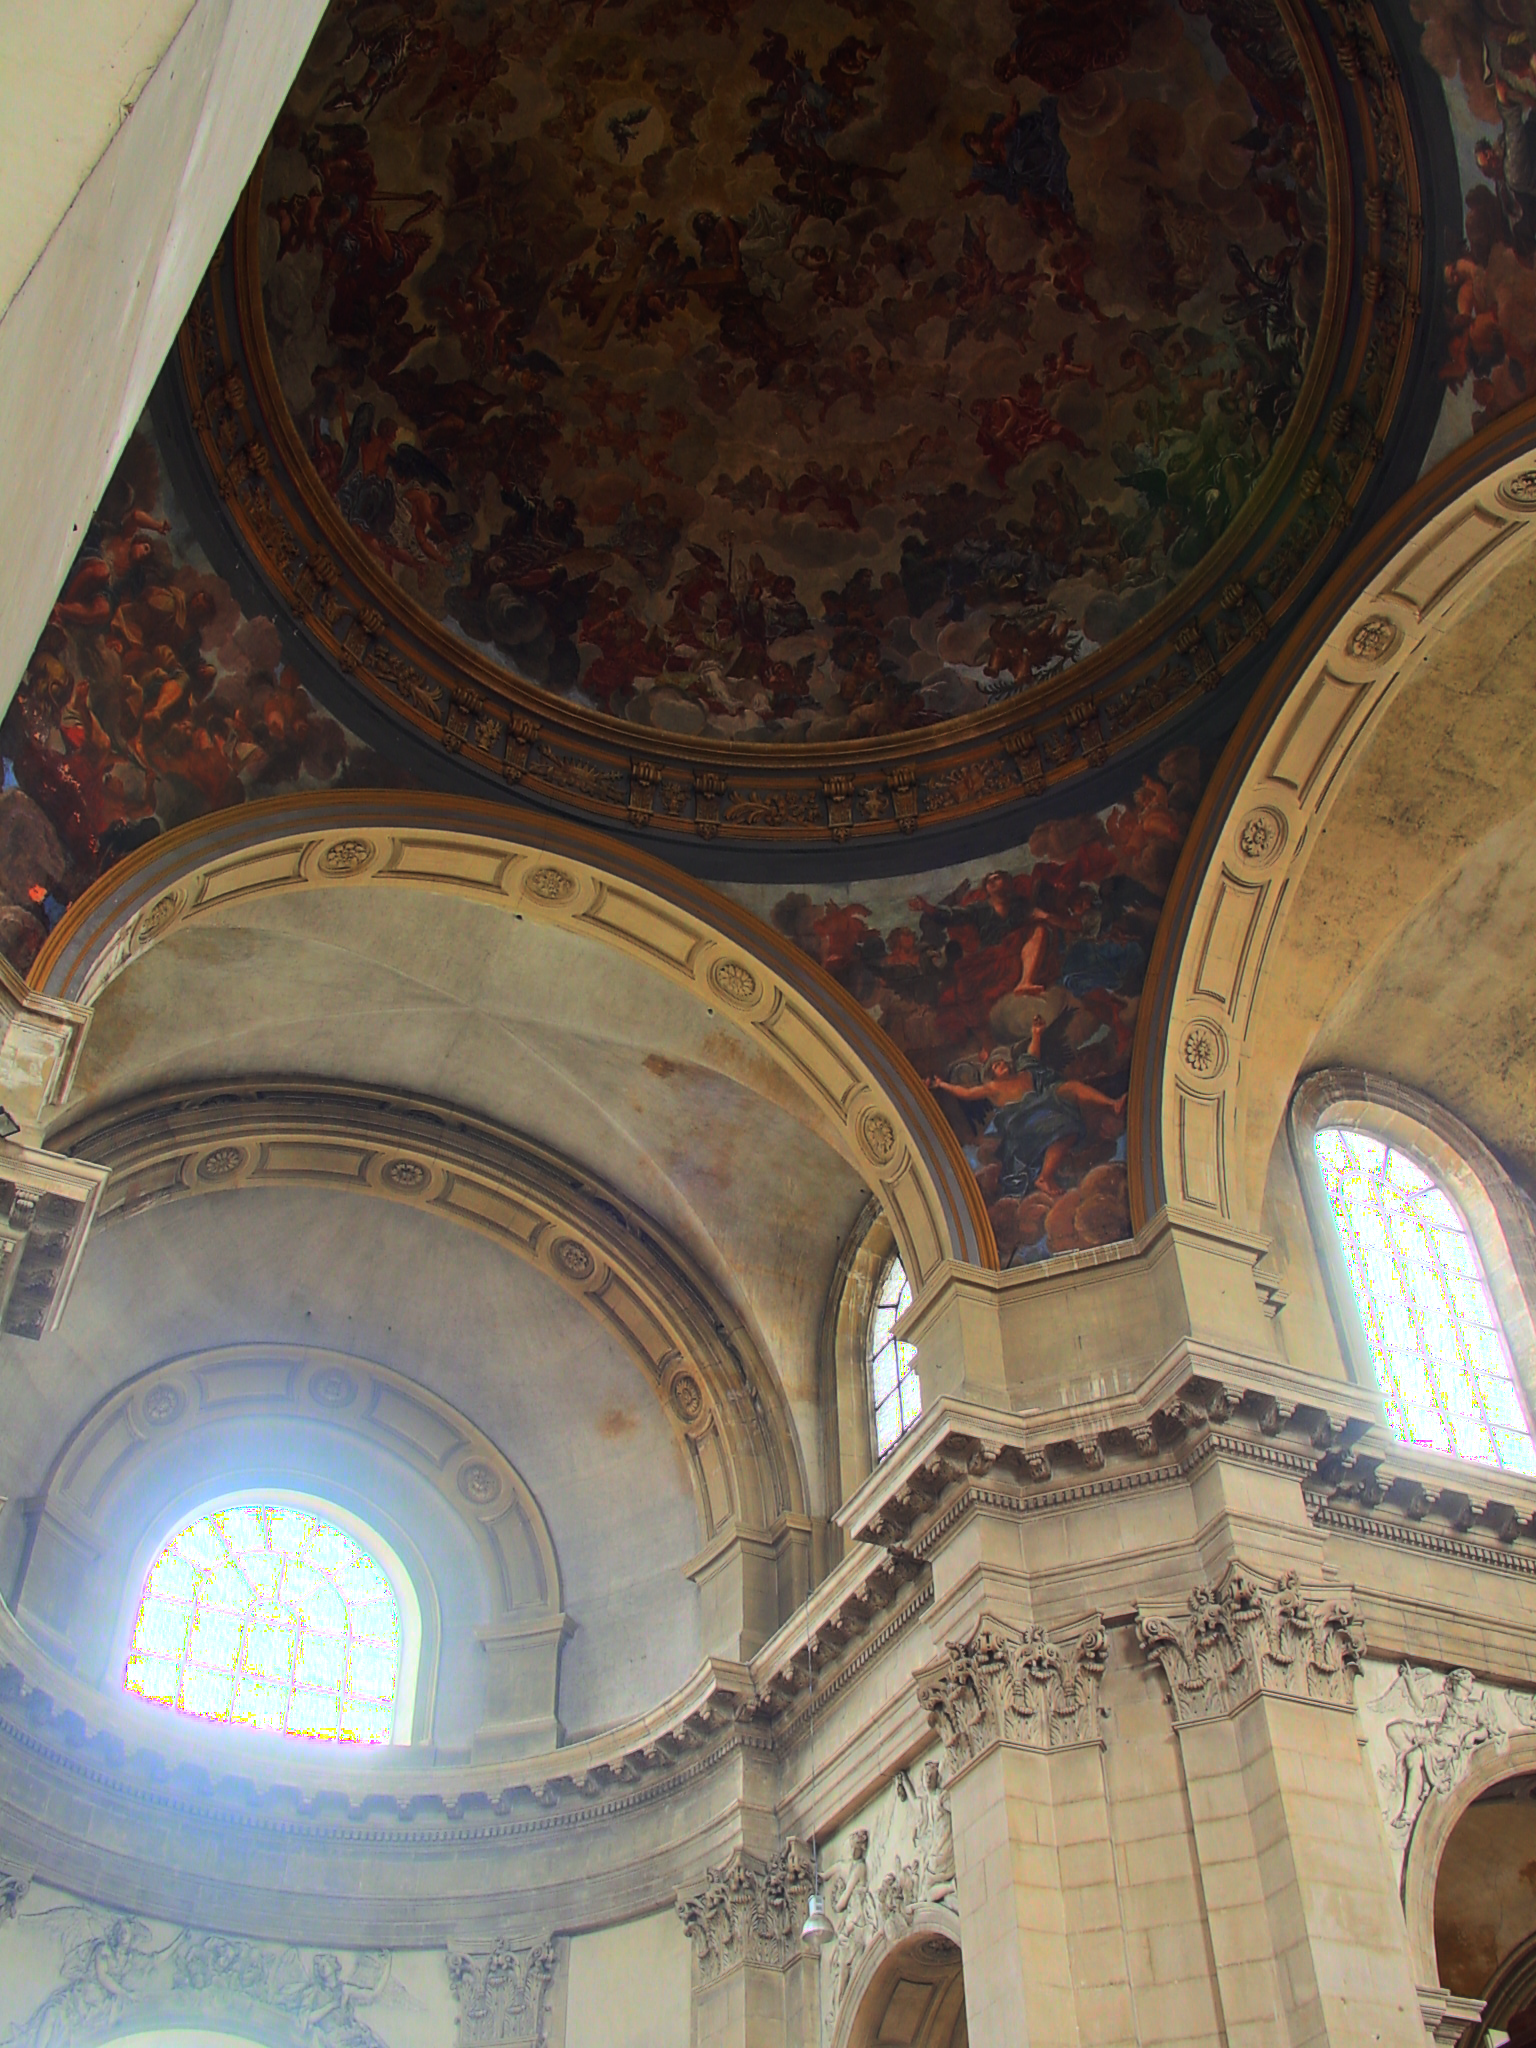
\includegraphics[width=.3\linewidth,valign=m]{churchDrago03.png} &
    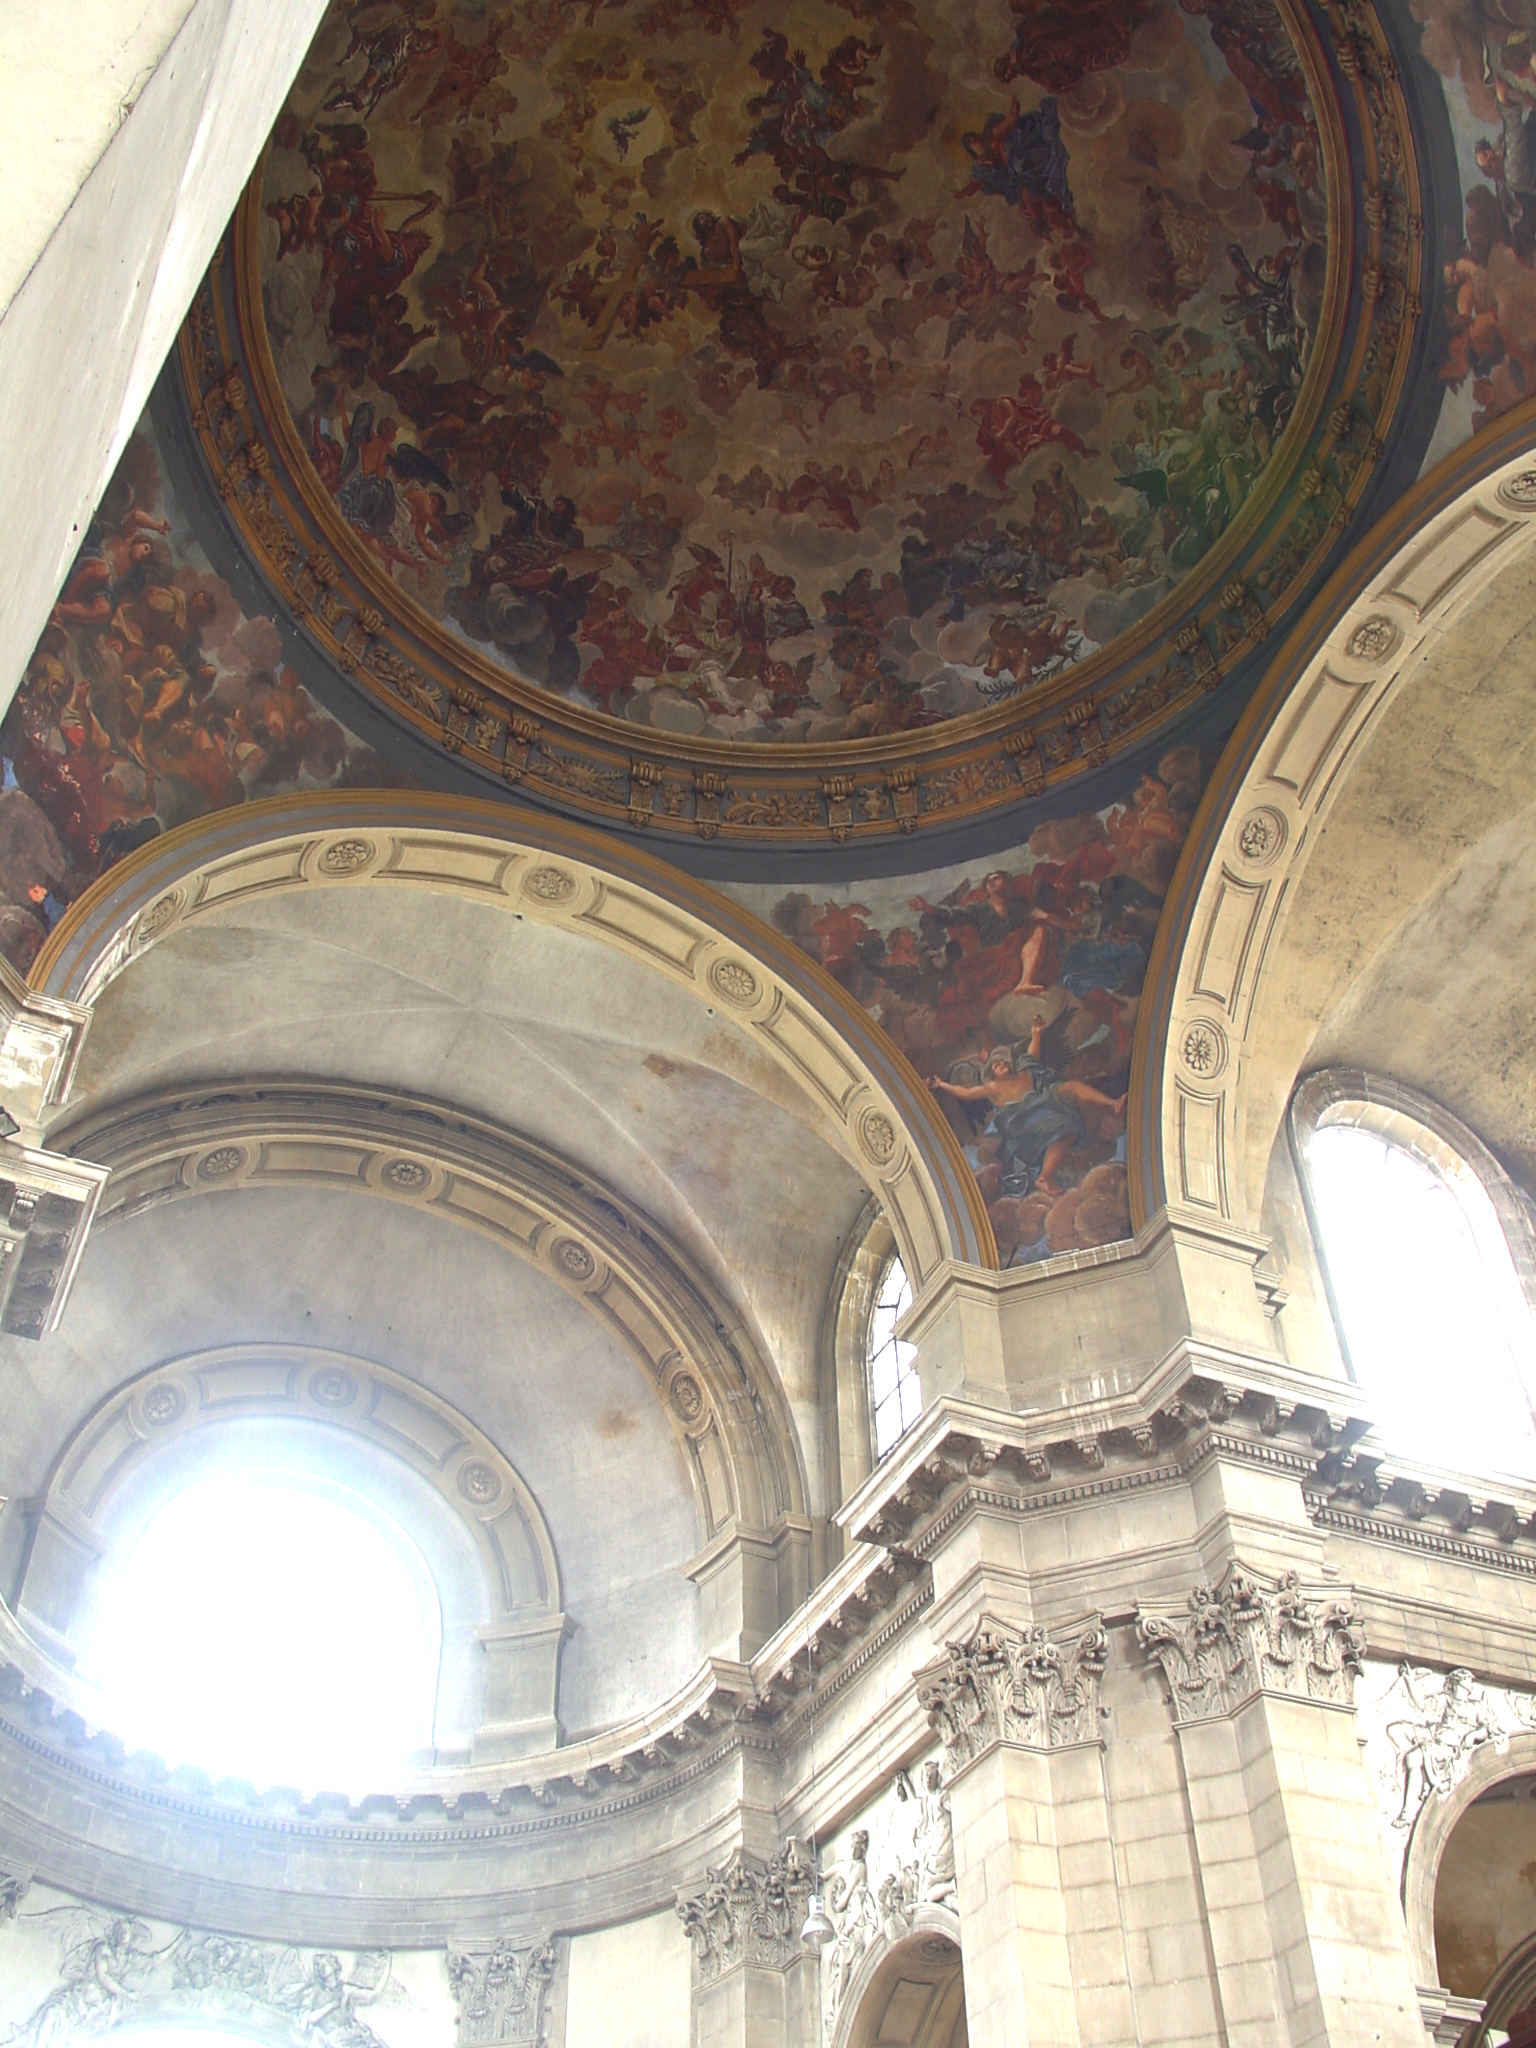
\includegraphics[width=.3\linewidth,valign=m]{churchWard94.png} \\
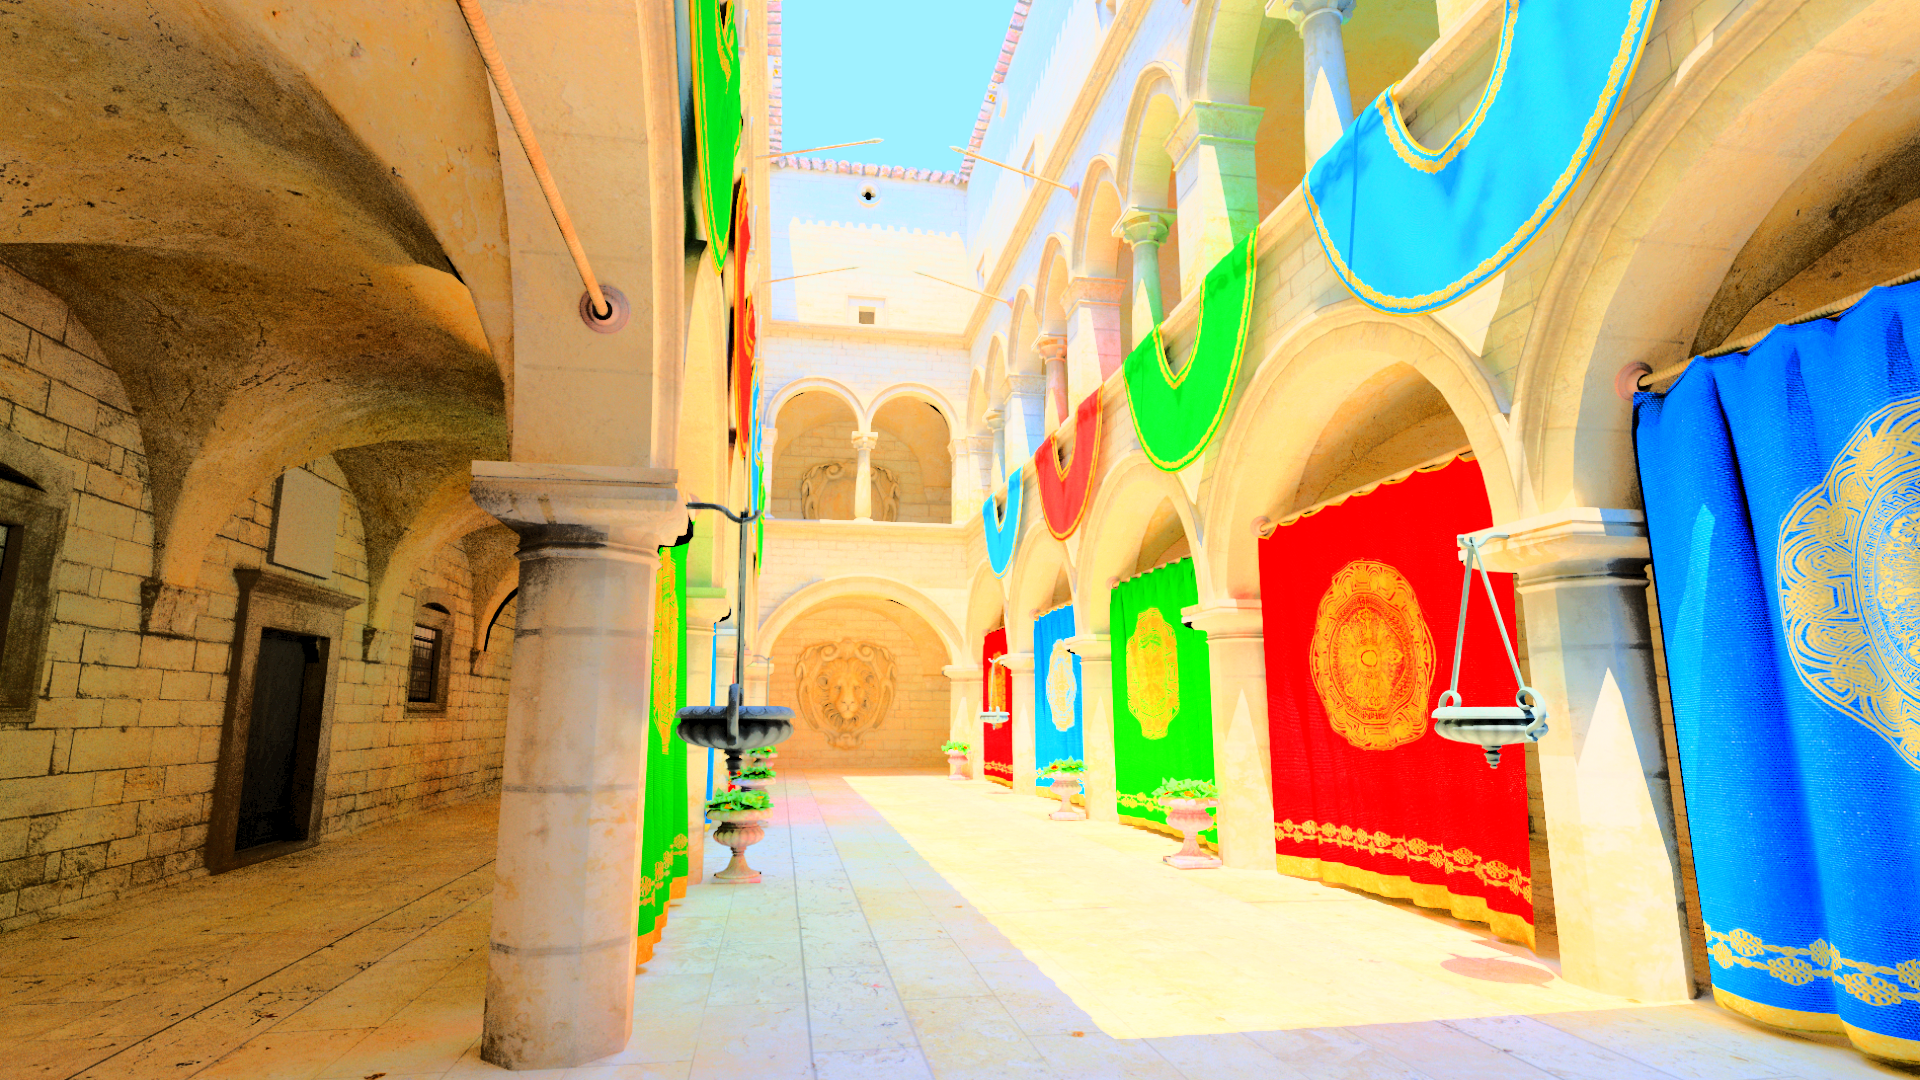
\includegraphics[width=.3\linewidth,valign=m]{buildingKhan20.png} &
    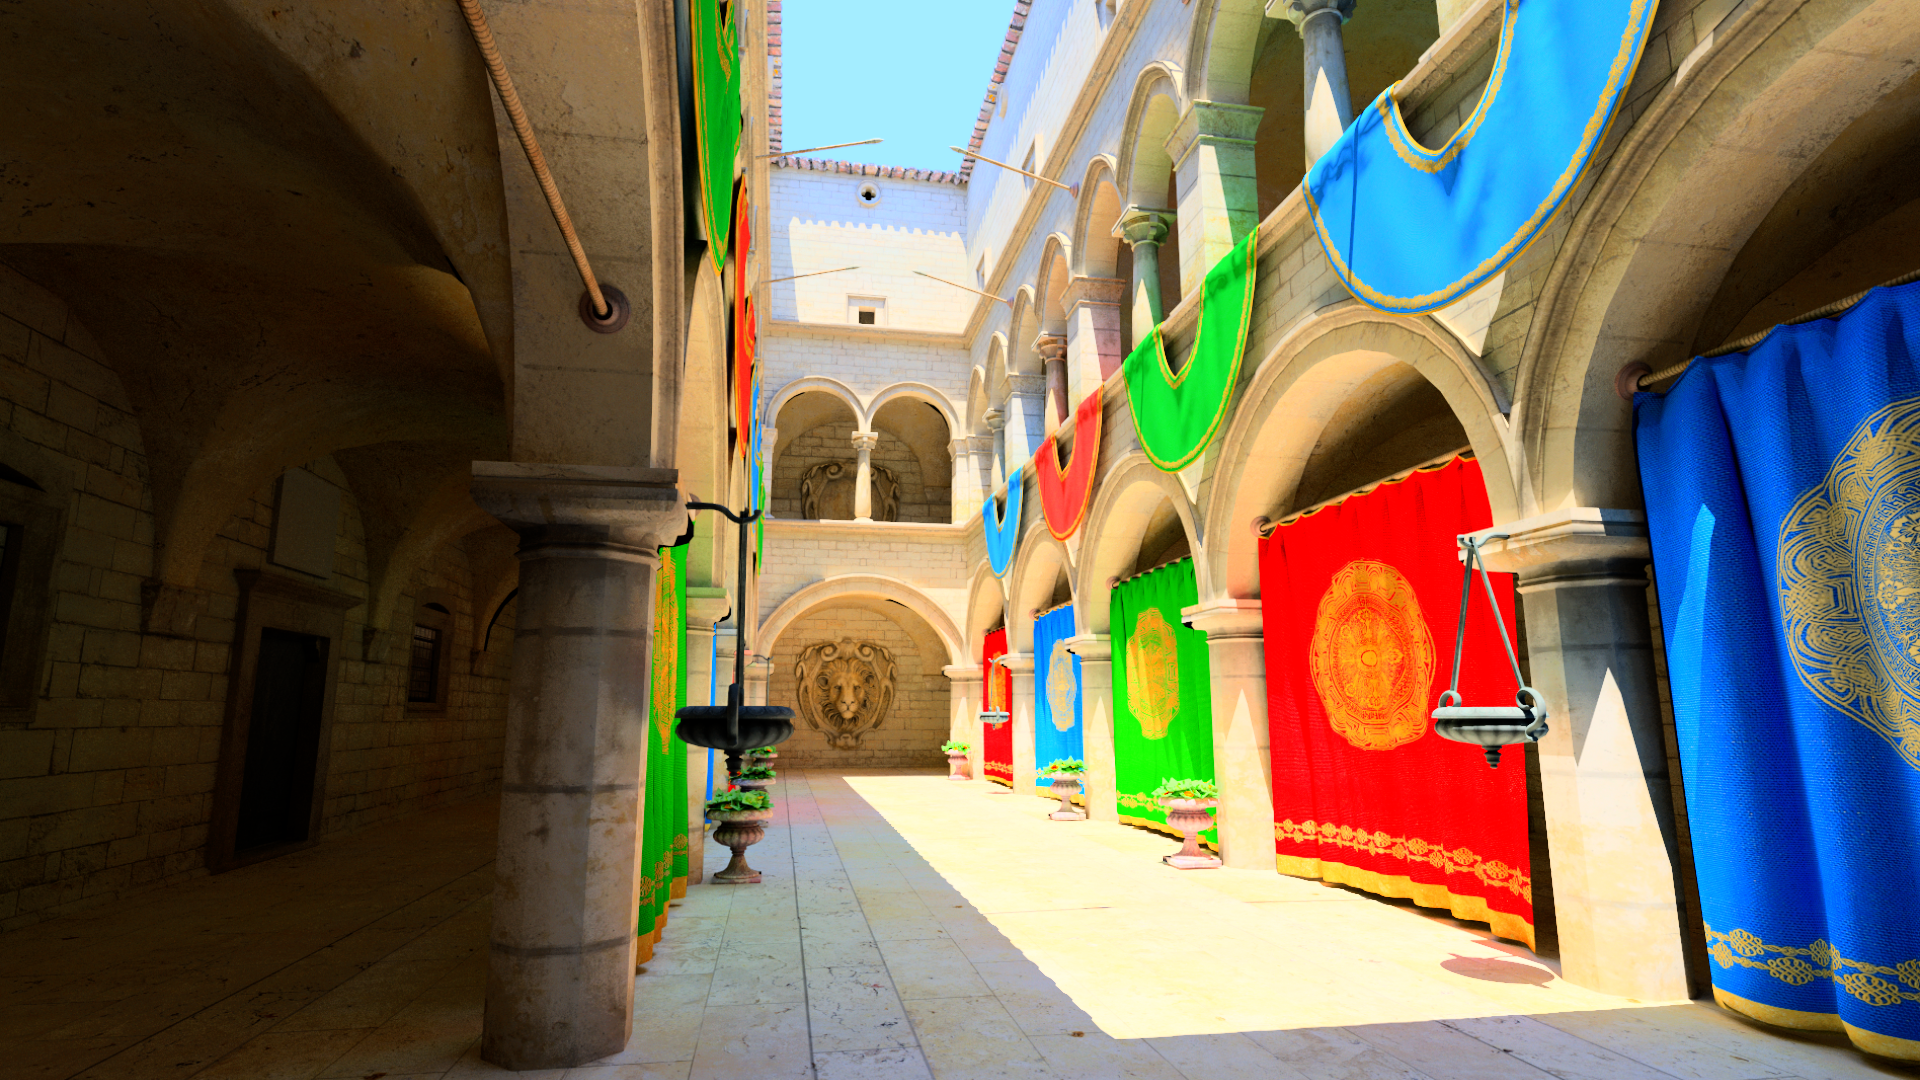
\includegraphics[width=.3\linewidth,valign=m]{buildingDrago03.png} &
    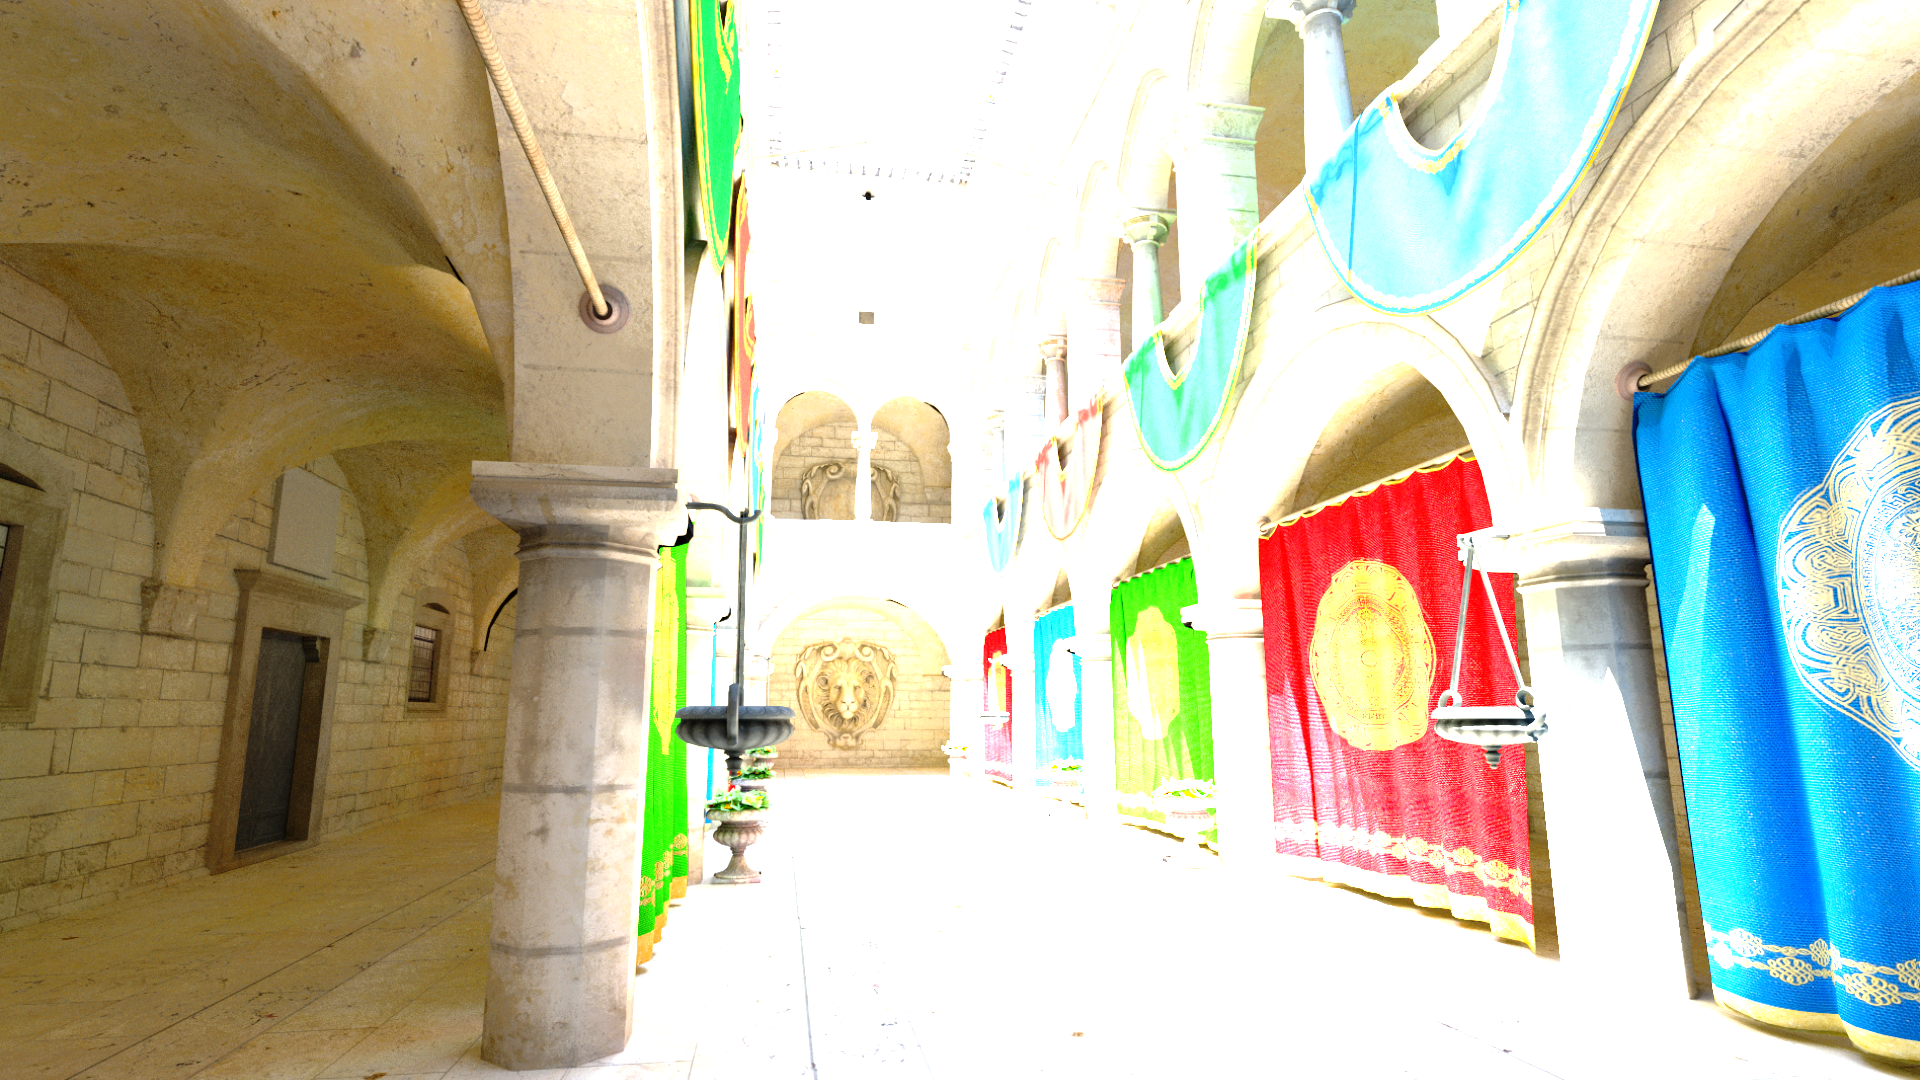
\includegraphics[width=.3\linewidth,valign=m]{buildingWard94.png}\\
\includegraphics[width=.3\linewidth,valign=m]{cornell_boxKhan20.png} &
    \includegraphics[width=.3\linewidth,valign=m]{cornell_boxDrago03.png} &
    \includegraphics[width=.3\linewidth,valign=m]{cornell_boxWard94.png}\\
\end{tabular}

\subsection{Uživatelská studie}

Poznatky získané testováním.


\section{Závěr}

\bibliographystyle{acm}
\bibliography{report}

\end{document}
